\documentclass[titlepage]{article}
\usepackage{fullpage}
\usepackage{graphicx}

\renewcommand{\thesection}{\Roman{section}}

\begin{document}

\title{17-614 Formal Methods\\[1ex] Project: Structural Modeling}
\author{
	{\Large\textbf{Team 16}}\\[3ex]
	yashanan\\[1ex] salonisi\\[1ex] halkhala\\[1ex] ktakayam}
\date{\today}
\maketitle

\newpage

\section{Task 1}
\subsection{Include an object model diagram for your system.}

Below is the final version of our object model diagram. Note that the privacy levels in the below model are singleton sets, so we have used rounded corners to represent them.

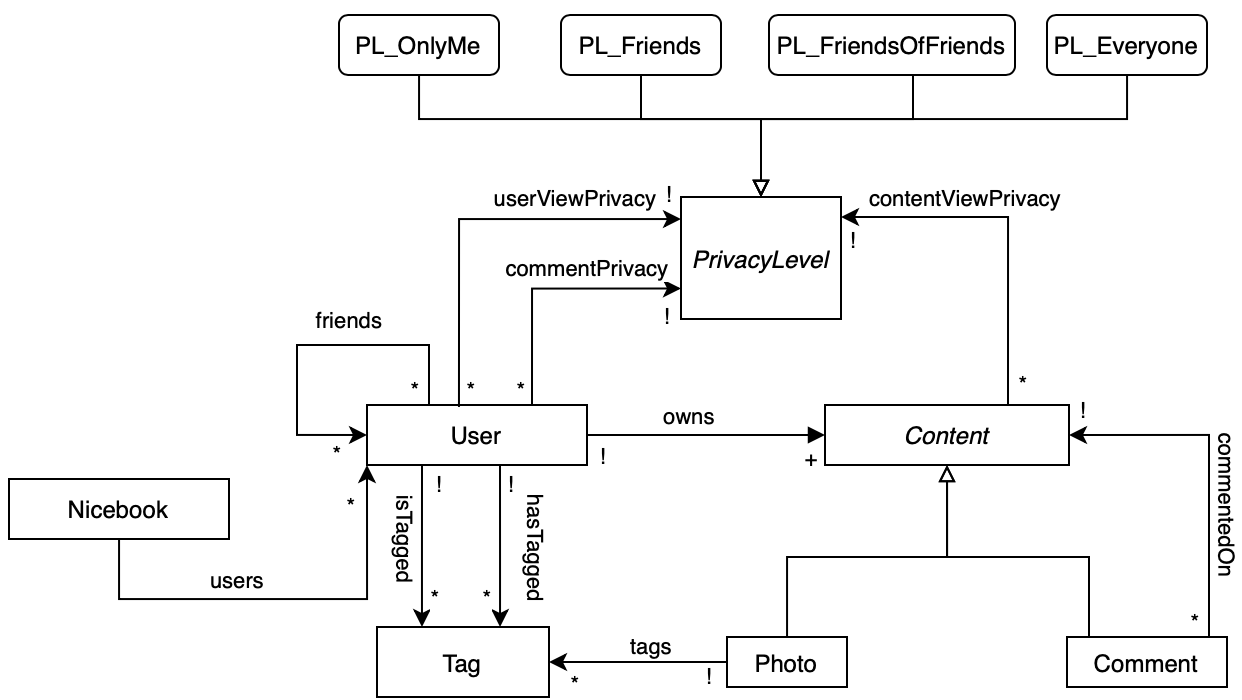
\includegraphics[width=6in]{images/single_model.png}

However, this model holds true only for a ‘snapshot’ of a single Nicebook. Below is the true model (that always holds), where we have redefined some object constraints to accommodate multiple Nicebook situations that arise when modeling actions (see section II.2.2). For e.g., some Content can be owned by two different users, given that they belong to different Nicebooks - a situation that arises during addPhoto when we need to copy a User to preserve all their existing Content.

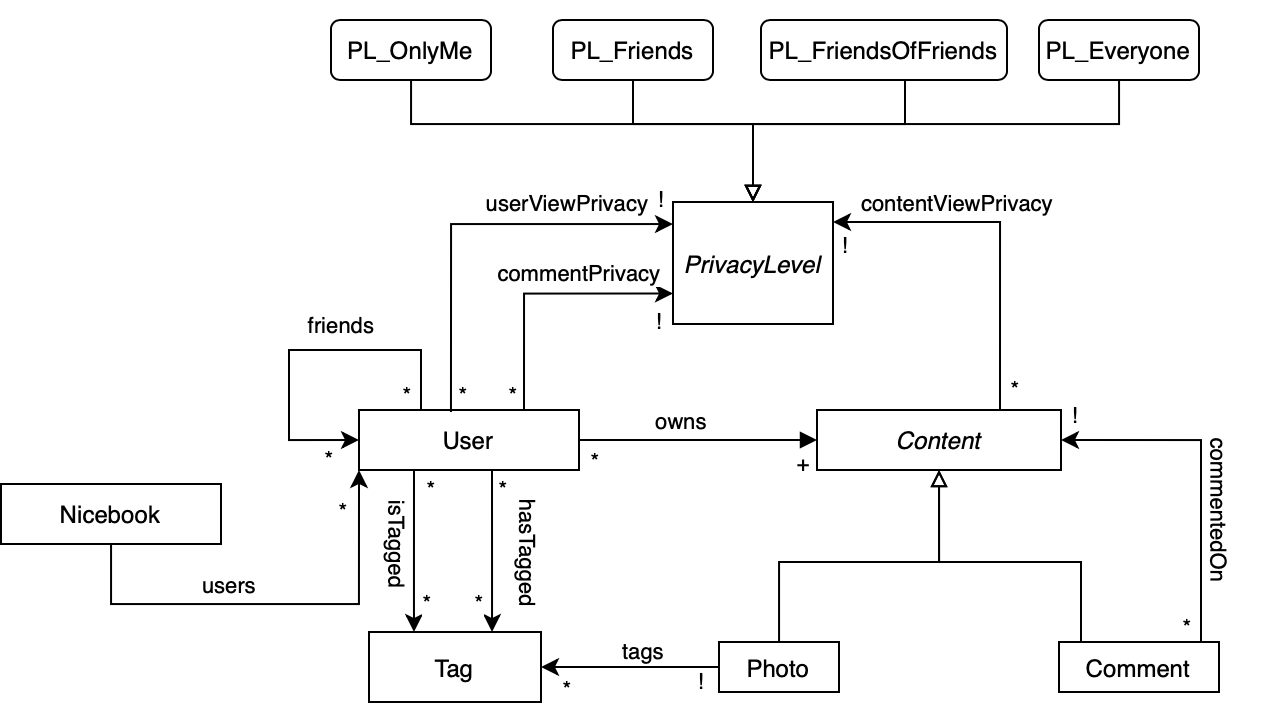
\includegraphics[width=6in]{images/true_model.png}

\subsection{Describe any decisions that your team made in resolving ambiguities in the English document. Also describe alternatives you considered and rejected.}

The decisions we made during the modeling process fall roughly into two categories: “Feature decisions” and “Internal modeling decisions”.
\subsubsection{Feature Decisions}
These are decisions we made regarding features that are exposed to the users.
\begin{enumerate}
\item\textbf{Privacy Settings}\\
There are three types of privacy settings defined in the project specification:
\begin{enumerate}
	\item Each piece of content owned by a user is associated with a privacy level that determines who can view that content on the user’s account.
	      \begin{enumerate}
		      \item We have defined a relationship contentViewPrivacy: Content $\rightarrow$ PrivacyLevel which is a content-specific setting that controls who related to the user can view user-owned content.
	      \end{enumerate}
	\item Each user has a setting that controls who can view content that is published on the user’s account by other users.
	      \begin{enumerate}
		      \item We assume that comments posted (both direct and nested) on user-owned content are considered content published by other users on the user’s account.
		      \item We have defined a relationship userViewPrivacy: User $\rightarrow$ PrivacyLevel which is a user-specific setting that controls viewing privileges for comments attached to user-owned content.
	      \end{enumerate}
	\item Each user has a setting that controls who can add a comment to content that is owned by the user.
	      \begin{enumerate}
		      \item We have defined a relationship commentPrivacy: User $\rightarrow$ PrivacyLevel which is a user-specific setting that controls who can comment on user-owned content.
	      \end{enumerate}
\end{enumerate}
\item\textbf{Content Viewing Priveleges}
\begin{enumerate}
	\item The getContentsInState[s: Nicebook] function returns the set of Content that belongs to the state s. A Content instance belongs to a state if the owner of the content as well as the owners of all parent contents (if any) belong to the state. In the below example, Comment belongs to S1 in the left state-chart since its user as well as the owner of its parent Content (Photo) belong to the state S1. However, in the right diagram, the owner of Comment belongs to S1, but since the owner of its parent Content does not belong to S2, Comment does not belong to S1 in the right diagram.

	      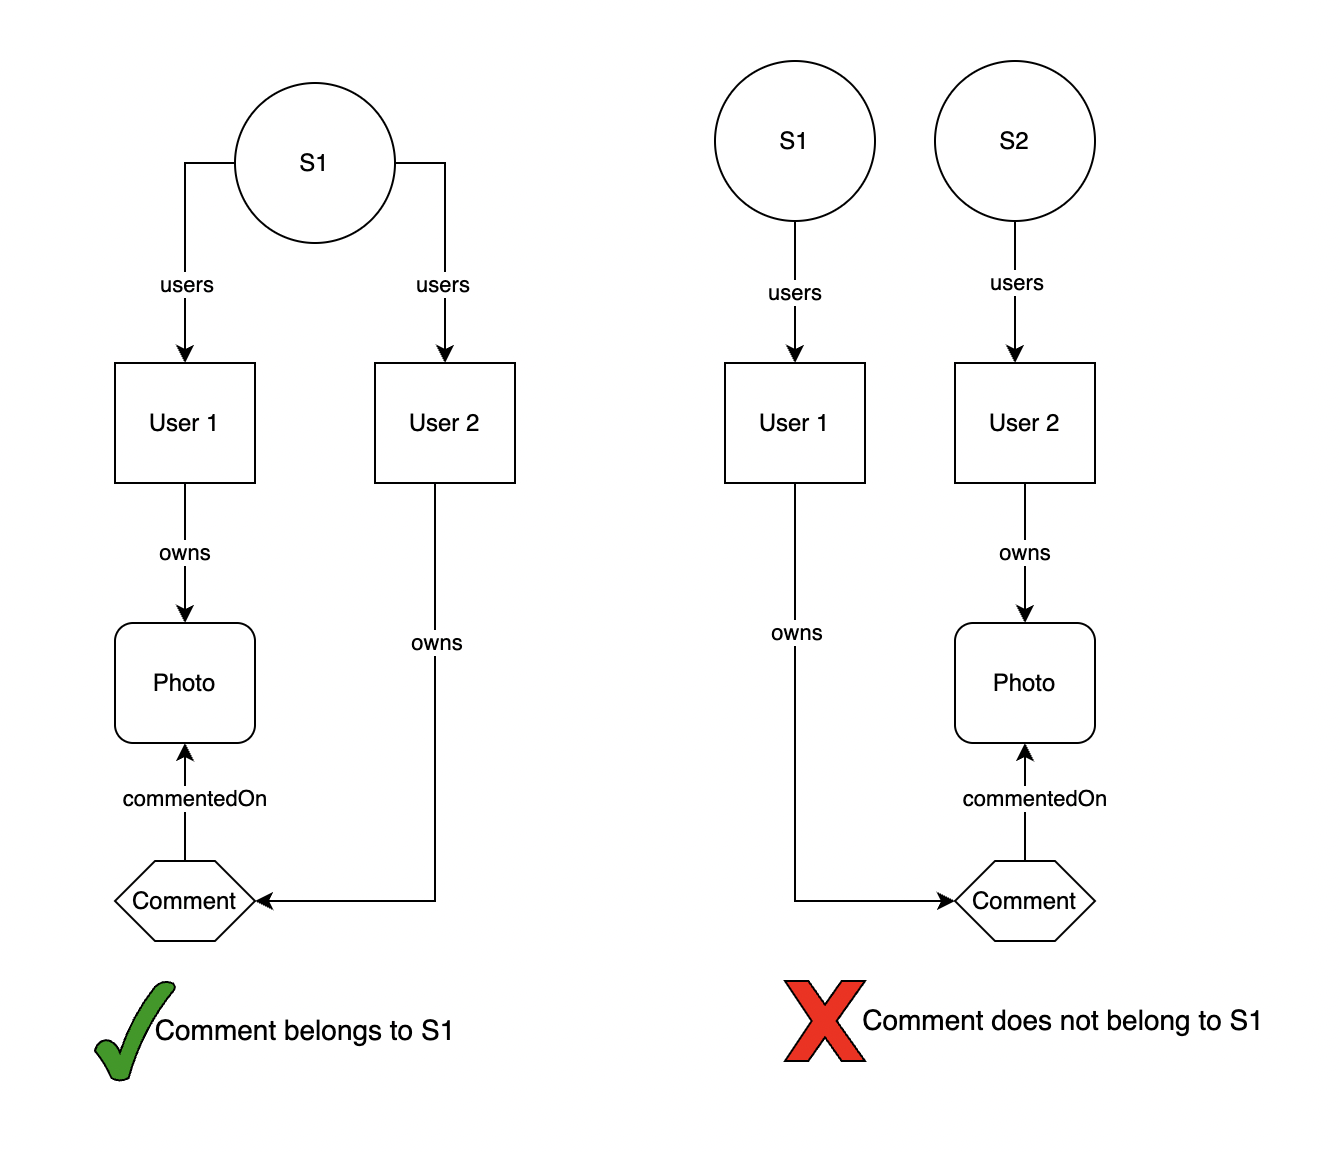
\includegraphics[width=6in]{images/content_view_1.png}

	\item We have defined a function called canView which takes a User instance and a Nicebook instance (representing the state) as arguments and returns the set of Contents that the user can view in a given state. A user can view Content if all of the following conditions hold:

	      \begin{enumerate}
		      \item The content belongs to the state
		      \item The user has viewing privileges for the said content as defined in the contentViewPrivacy relation.
		      \item If the user has parent elements, the user must have privileges to view the “children” elements of parent elements. This is defined in the userViewPrivacy relation.
		      \item All the above conditions must satisfy for the content at hand as well as all parent elements of the said content – In short, a content can only be viewed if all its parent contents can also be viewed.
	      \end{enumerate}
	      \item\textbf{Exception: A user can view all comments and nested comments on content owned by him/her regardless of the contentViewPrivacy and userViewPrivacy settings defined by those comments and owners of those comments respectively.}
\end{enumerate}
\item\textbf{Commenting Priveleges}
\begin{enumerate}
\item We have defined a function canCommentOn[u: User, s : Nicebook] which returns the set of Contents that the user can comment on. A user can comment on a content if the following conditions hold:
\begin{enumerate}
	\item The user can view the content as defined in the canView function.
	\item The user has commenting privileges as defined by the content owner in the commentPrivacy relation.

	\item The above conditions must hold true for all its parent content elements, if any.
\end{enumerate}
\item\textbf{Exception: A user can comment on comments and nested comments that are attached to contents owned by the user, regardless of the commentPrivacy settings set up by owners of those nested comments.}
\item\textbf{Operation Priveleges}
\begin{enumerate}
	\item \underline{Adding a photo}: Any user can perform this action. When a photo is added by a user, the relationship “owns” is established between the user and the photo.
	\item \underline{Deleting a photo}: A photo can be deleted by the owner of the photo only.
	\item \underline{Adding a comment}: To add a comment on an instance of Content, the following conditions must hold true:
	      \begin{enumerate}
		      \item The user must have commenting privileges on content as defined in the canCommentOn function.
	      \end{enumerate}
	\item \underline{Deleting a comment}: In order to delete a comment, either of the following must hold:
	      \begin{enumerate}
		      \item The user is the owner of the comment
		      \item The user is the owner of one of the parent elements of the said comment.
		            \end {enumerate}
		      \item \underline{Adding a tag}: A user can tag another user on a photo if the following holds true:
		            \begin{enumerate}
			            \item Both users have the privilege of viewing the Photo.
			            \item The two users are friends in the same state
		            \end{enumerate}
		      \item \underline{Removing a tag}: A user can remove a tag if any one or more of the following conditions holds true:
		            \begin{enumerate}
			            \item The user is the owner of the Photo which is tagged.
			            \item The user is tagged on a Photo and wants to remove his/her own tag from the Photo.
			            \item The user has tagged another user on a Photo and now wants to remove this tag.
		            \end{enumerate}
	      \end{enumerate}
	      \end {enumerate}
\end{enumerate}

\subsubsection{Internal Modeling Decisions}
These are internal alloy-related modeling decisions that do not affect what a user sees but how we choose to model our system.
\begin{enumerate}
	\item \textbf{Modeling Tags}
\end{enumerate}

\subsection{Describe any invariants that are not explicitly mentioned in the given document but were discovered during the modeling process.}
\subsection{Describe an invariant that was violated by an operation in your model and how it was fixed.}
\subsection{List the scope used for the analysis of invariant preservation. Why did you choose this scope, and why do you
	think it is sufficient?}

\section{Task 2}
\subsection{Define an Alloy function called canView, which takes at least one parameter that represents some user in the
	social network, and returns the set of all content that can be viewed by that user. You may use any number of
	helper predicates or functions to define canView.}
\subsection{You will use canView to check whether it is possible for a user to access a piece of content against the intent of the owner. In particular, we say that a privacy violation has occurred if a user is able to view a piece of content without adhering to the privacy level that is assigned to the content by its owner. For example, suppose that Alice
	and Bob are not friends, and Alice has a photo that is assigned privacy setting Friends; if Bob is able to view the
	photo, this would be considered a privacy violation. Define an Alloy assertion called NoPrivacyViolation
	to check that no such violation is possible.}
\subsection{Does your model satisfy NoPrivacyViolation? If so, explain why. If not, include a counterexample that
	demonstrates a violation, and suggest a modification to the design of privacy settings in Nicebook. Describe
	any alternatives you considered and rejected, along with justifications for your decision.}

\section{Task 3}
\subsection{What are the strengths and weaknesses of Alloy and its tool, the Alloy Analyzer?}
\subsection{Under what situations would you recommend its use (or not)? Why?}
\subsection{With respect to this notation, what is the single most-important future development that would be needed to
	make it more generally useful to practitioners?}
\end{document}
